\documentclass[12pt]{article}

\usepackage{amsmath,amssymb}
\usepackage{graphicx}
\usepackage{geometry}
\usepackage{setspace}
\usepackage{hyperref}
\usepackage{booktabs}

\geometry{margin=1in}
\onehalfspacing
\graphicspath{{figures/supplementary/}{figures/}}

\title{Fold-dependent slowing in mechanistic CSD}
\author{}
\date{}

\begin{document}
\maketitle

\renewcommand{\thetable}{S\arabic{table}}
\renewcommand{\thefigure}{S\arabic{figure}}

This supplement collects manuscript-adjacent details that are useful for review but too long for the main text: the full paired geometry sweep behind the mechanistic slowdown statistics, the exact representative-run outputs underlying manuscript Table~1, the atlas-patch sanity-check figure, and a narrow physiology-anchor check against published CSD speed and delay bands. The physiology-anchor items come from the reduced biophysical validation workflow and should be read as contextual support rather than as a direct fit of the multi-ion mechanistic surface model.

\section*{Supplementary Tables}

\begin{table}[t]
\centering
\caption{Full paired geometry sweep for the mechanistic surface electrodiffusion model. Each row compares the same geometry with dipole alignment disabled or enabled. The flat control is included as an internal specificity check and shows zero slowing.}
\label{tab:geometry_sweep}
\scriptsize
\resizebox{\textwidth}{!}{%
\begin{tabular}{@{}rrrrrrrrrrr@{}}
\toprule
Depth (mm) & $\sigma$ (mm) & Severity & Baseline speed & Dipole speed & Slowdown & Baseline delay & Dipole delay & Delay increase & Baseline $|V_e|$ & Dipole $|V_e|$ \\
 &  &  & (mm/min) & (mm/min) & (mm/min) & (s) & (s) & (s) & (mV) & (mV) \\
\midrule
0.0 & 1.5 & 0.000 & 3.623 & 3.623 & 0.000 & 64.3 & 64.3 & 0.0 & 19.43 & 19.43 \\
1.2 & 1.1 & 1.091 & 2.355 & 2.259 & 0.096 & 135.1 & 141.5 & 6.4 & 21.88 & 21.81 \\
1.2 & 1.5 & 0.800 & 2.368 & 2.239 & 0.128 & 130.3 & 139.9 & 9.6 & 21.54 & 21.68 \\
1.2 & 1.9 & 0.632 & 2.415 & 2.337 & 0.078 & 124.8 & 128.9 & 4.1 & 21.09 & 21.24 \\
1.8 & 1.1 & 1.636 & 2.603 & 2.485 & 0.118 & 135.2 & 141.8 & 6.6 & 22.11 & 22.01 \\
1.8 & 1.5 & 1.200 & 2.554 & 2.415 & 0.140 & 130.0 & 139.4 & 9.3 & 21.65 & 21.80 \\
1.8 & 1.9 & 0.947 & 2.556 & 2.439 & 0.117 & 124.5 & 130.4 & 5.9 & 21.14 & 21.03 \\
2.4 & 1.1 & 2.182 & 2.923 & 2.783 & 0.140 & 135.1 & 142.2 & 7.0 & 22.29 & 22.14 \\
2.4 & 1.5 & 1.600 & 2.802 & 2.646 & 0.156 & 129.8 & 138.6 & 8.8 & 21.75 & 21.90 \\
2.4 & 1.9 & 1.263 & 2.736 & 2.661 & 0.075 & 124.1 & 127.5 & 3.4 & 21.23 & 21.37 \\
3.0 & 1.1 & 2.727 & 3.287 & 3.129 & 0.158 & 135.1 & 142.2 & 7.0 & 22.44 & 22.18 \\
3.0 & 1.5 & 2.000 & 3.071 & 2.833 & 0.238 & 129.5 & 141.8 & 12.3 & 21.85 & 21.66 \\
3.0 & 1.9 & 1.579 & 2.898 & 2.816 & 0.082 & 123.6 & 126.8 & 3.2 & 21.32 & 21.45 \\
\bottomrule
\end{tabular}%
}
\end{table}

\begin{table}[t]
\centering
\caption{Exact representative-run outputs underlying manuscript Table~1 for the folded surface used in the main manuscript (fold depth 2.4~mm, $\sigma=1.5$~mm). Values are copied directly from the saved final representative run, not from a rerun. The full coupled run is retained only as an exploratory sensitivity analysis because vascular feedback changes the excitability regime.}
\label{tab:representative_metrics}
\scriptsize
\resizebox{\textwidth}{!}{%
\begin{tabular}{@{}lrrrrrrrrrr@{}}
\toprule
Case & $dt$ (s) & Speed (mm/min) & E1 arrival (s) & E2 arrival (s) & Delay (s) & Max $|V_e|$ (mV) & Max $K_e$ (mM) & Max swelling & Min oxygen & Min perfusion \\
\midrule
Baseline mechanistic & 0.04996995735874618 & 2.5582349901822656 & 30.681553818270157 & 161.20308243931518 & 130.52152862104504 & 18.987306193669685 & 35.6329071567077 & 1.4998735073093261 & 1.0 & 0.6 \\
Dipole-aligned mechanistic & 0.04996995735874618 & 2.475787705816325 & 30.681553818270157 & 165.3505889000911 & 134.66903508182097 & 19.50089527429308 & 35.61903013535566 & 1.4998731422865321 & 1.0 & 0.6 \\
Full coupled sensitivity & 0.04996995735874618 & 3.546505127010437 & 30.431704031476425 & 124.52513373799549 & 94.09342970651906 & 12.95984978092811 & 32.865620644529656 & 1.4998601120671369 & 0.2 & 0.25 \\
\bottomrule
\end{tabular}%
}
\end{table}

The speed bands summarized in Table~\ref{tab:physiology_anchor} and Fig.~\ref{fig:physiology_anchor} are the same published experimental and clinical ranges discussed in the main manuscript. In the present supplement they are included only as a narrow contextual check that accepted scalar and tensor validation cases remain within published speed regimes while preserving the tensor-faster-than-scalar ordering.

\begin{table}[t]
\centering
\caption{Accepted-candidate physiology anchor from the reduced biophysical validation sweep. This table is included as a contextual range check against published CSD speed and delay bands, not as a direct validation of the multi-ion mechanistic surface model.}
\label{tab:physiology_anchor}
\small
\resizebox{\textwidth}{!}{%
\begin{tabular}{@{}llllll@{}}
\toprule
Metric & Range (mm/min) & Mean & Within 2.0--5.0 & Within 1.7--9.2 & Within 2.5--4.5 \\
\midrule
Control & 3.000--3.000 & 3.000 & 63/63 & 63/63 & 63/63 \\
Scalar & 2.606--2.750 & 2.635 & 63/63 & 63/63 & 63/63 \\
Tensor & 2.683--2.792 & 2.706 & 63/63 & 63/63 & 63/63 \\
Tensor - scalar & 0.042--0.077 & 0.071 & -- & -- & -- \\
\midrule
Scalar downstream delay (s) & 0.0--16.2 s & 12.8 s & \multicolumn{3}{l}{Within 10--30 s band: 54/63} \\
\bottomrule
\end{tabular}%
}
\end{table}

\clearpage
\section*{Supplementary Figures}

\begin{figure}[t]
\centering
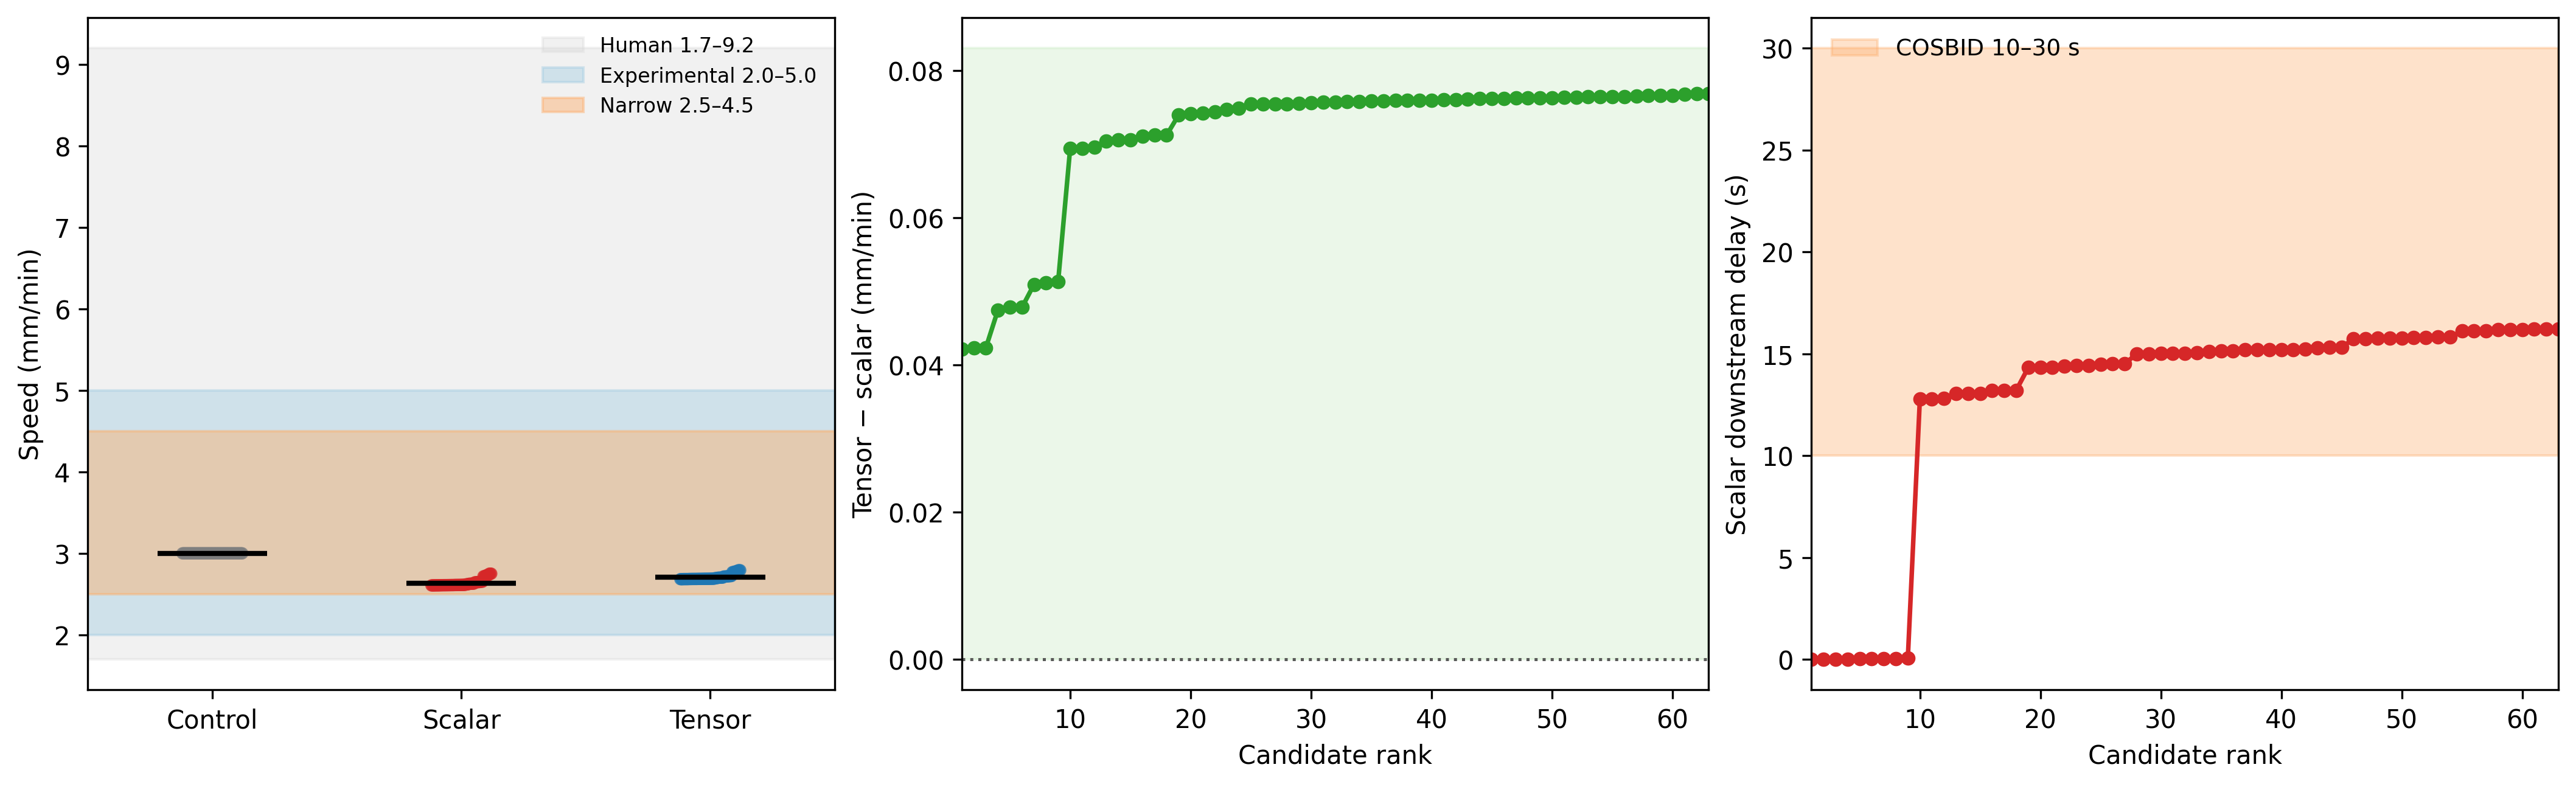
\includegraphics[width=\textwidth]{fig_physiology_anchor.png}
\caption{Physiology-anchor summary for the accepted reduced-biophysical validation cases. Shaded or annotated ranges denote the same broad published CSD speed and delay bands discussed in the main manuscript. The figure is included as a contextual supplement and should not be interpreted as a direct waveform-level validation of the mechanistic surface electrodiffusion model.}
\label{fig:physiology_anchor}
\end{figure}

\begin{figure}[htbp]
\centering
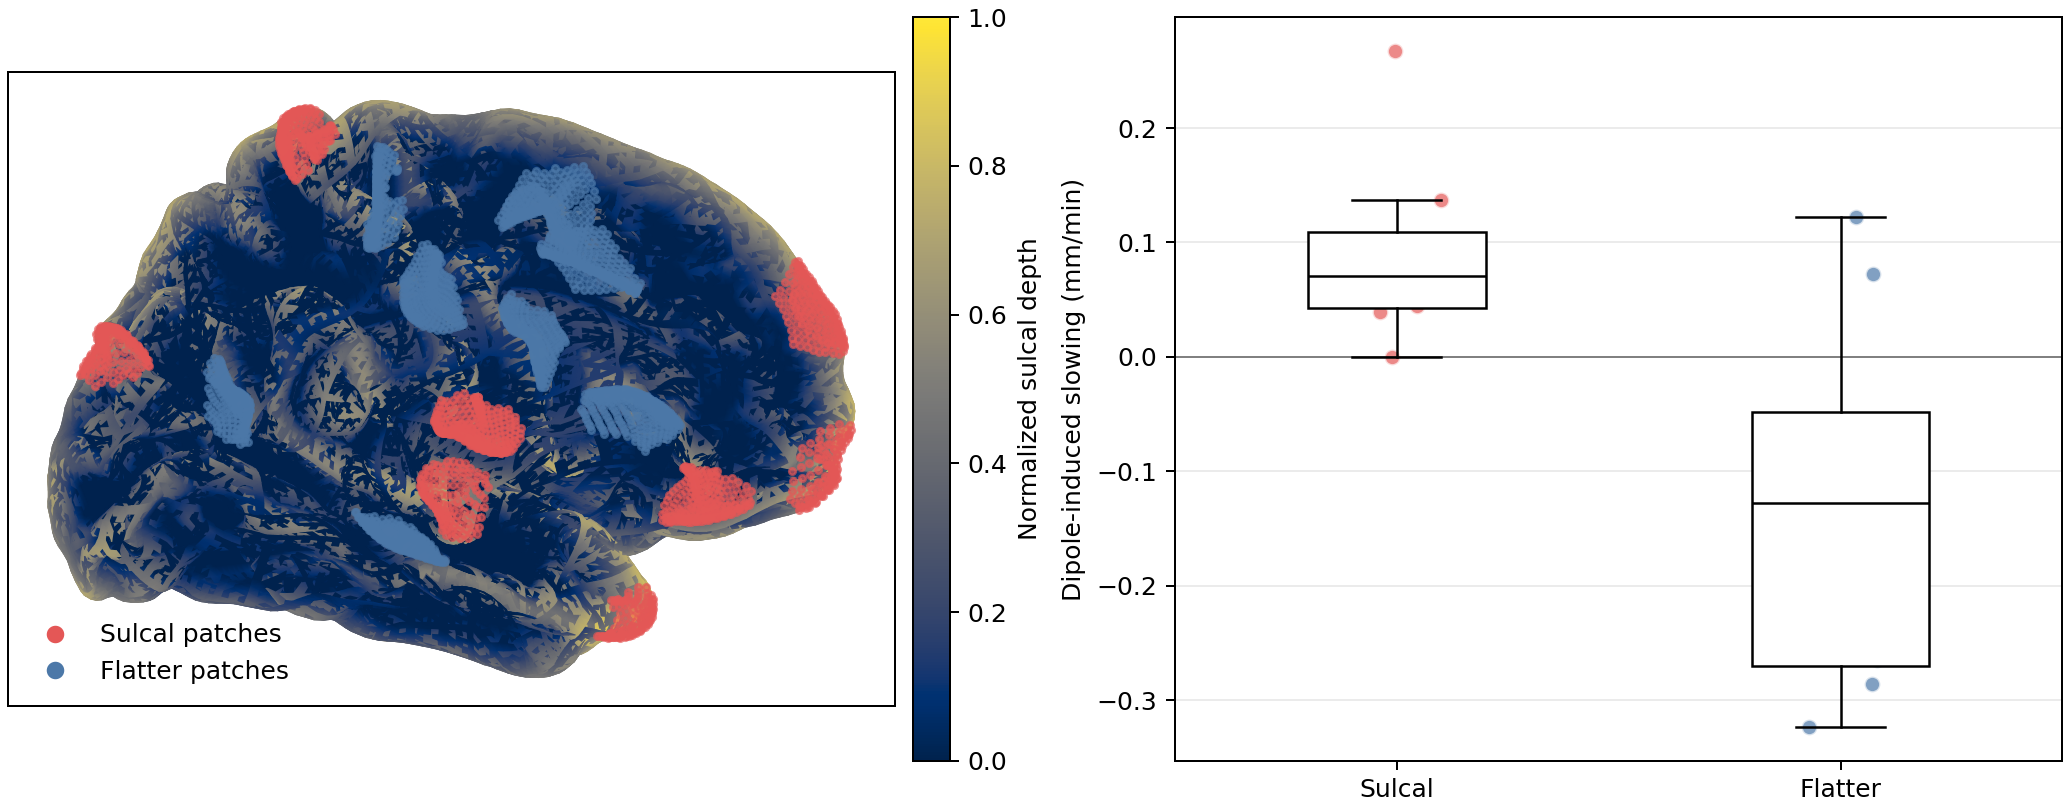
\includegraphics[width=\textwidth]{mechanistic_atlas_patch_qc.png}
\caption{Atlas-based multi-patch sanity check used as a geometry-specific supplement to the main mechanistic results. Left, the fsaverage6 left-hemisphere midthickness surface with the $N=8$ selected sulcal and $N=8$ flatter matched patches overlaid on the normalized sulcal-depth map. Right, the distributions of dipole-induced propagation slowing for each patch category. The consistent positive slowdown on sulcal patches supports the main mechanistic results, whereas flatter patches (which still possess local structural curvature) yield inverted effects. This figure remains supplementary because it functions as an atlas-based sign-check rather than a full subject-specific human validation study.}
\label{fig:atlas_sanity_check}
\end{figure}

\end{document}
